

\section*{\huge{Supplemental Information}}

\renewcommand{\thefigure}{S\arabic{figure}}
\renewcommand{\theequation}{S\arabic{equation}}
\renewcommand{\thetable}{S\arabic{table}}
\setcounter{equation}{0}
\setcounter{figure}{0}
\setcounter{table}{0}


% Note: this should go into a separate document eventually

\section*{Matrix derivatives in quantitative genetics equations}

As in the main text, $^{\textrm{T}}$ indicates transposition,
multiplication between matrices is always matrix multiplication, and
bold face indicates a matrix.
Also note that both $\mathbf{C}$ and $\mathbf{D}$ are symmetrical,
so $\mathbf{C} + \mathbf{C}^{\textrm{T}} = 2 \; \mathbf{C}$ and
$\mathbf{D} + \mathbf{D}^{\textrm{T}} = 2 \; \mathbf{D}$.




\subsection*{Jacobian matrix}

The $n(q+1) \times n(q+1)$ Jacobian matrix consists of 

\begin{itemize}
\item $n^2$ blocks of size $q \times q$ containing
    $\partial \mathbf{v}_{i,t+1} / \partial \mathbf{v}_{\zeta,t}$
\item $n^2$ blocks of size $1 \times q$ containing
    $\partial \mathbf{v}_{i,t+1} / \partial N_{\zeta,t}$
\item $n^2$ blocks of size $q \times 1$ containing
    $\partial N_{i,t+1} / \partial \mathbf{v}_{\zeta,t}$
\item $n^2$ blocks of size $1 \times 1$ containing
    $\partial N_{i,t+1} / \partial N_{\zeta,t}$
\end{itemize}


for all $i \in \{ 1, \: \ldots \, , \: n \}$
and $\zeta \in \{ 1, \: \ldots \, , \: n \}$.


The partial derivatives of species $i$ axes at time $t+1$ with respect
to species $i$ axes at time $t$ are

\begin{equation*}
\begin{split}
    \frac{ \partial \, \mathbf{v}_{i,t+1} }{ \partial \, \mathbf{v}_{i,t} } &=
        \frac{ \partial \, \mathbf{v}_{i,t} }{ \partial \, \mathbf{v}_{i,t} } +
        2 \; \sigma_A^2
        \left(
            \frac{ \partial \;
                \alpha_0 \; 
                \left( 
                    \sum_{j \ne i}^{n}{ N_{j,t} \, \textrm{e}^{
                    - \mathbf{v}_{j,t}^{\textrm{T}}
                    \mathbf{D} \mathbf{v}_{j,t} } }
                \right) \;
                    \textrm{e}^{-\mathbf{v}_{i,t}^{\textrm{T}} \mathbf{v}_{i,t}} \,
                    \mathbf{v}_{i,t}^{\textrm{T}}}{\partial \; \mathbf{v}_{i,t} } -
            \frac{ \partial \; f \, \mathbf{v}_{i,t}^{\textrm{T}} \mathbf{C}}{\partial \; \mathbf{v}_{i,t} }
        \right) \\
    &=
        \mathbf{I} +
        2 \; \sigma_A^2
        \left[
            \alpha_0
            \left( 
                \sum_{j \ne i}^{n}{ N_{j,t} \, \textrm{e}^{
                - \mathbf{v}_{j,t}^{\textrm{T}}
                \mathbf{D} \mathbf{v}_{j,t} } }
            \right) \,
            \left(
                \textrm{e}^{-\mathbf{v}_{i,t}^{\textrm{T}} \mathbf{v}_{i,t}} +
                \frac{ \partial \;
                        \textrm{e}^{-\mathbf{v}_{i,t}^{\textrm{T}} \mathbf{v}_{i,t}}
                        }{\partial \; \mathbf{v}_{i,t} } \, \mathbf{v}_{i,t}^{\textrm{T}}
            \right) -
            f \, \mathbf{C}^{\textrm{T}}
            \right] \\[2ex]
    \frac{ \partial \, \mathbf{v}_{i,t+1} }{ \partial \, \mathbf{v}_{i,t} } &= \mathbf{I} + 2 ~ \sigma_A^2 ~
        \left[
            \alpha_0 
            \left( 
                \sum_{j \ne i}^{n}{ N_{j,t} \, \textrm{e}^{
                - \mathbf{v}_{j,t}^{\textrm{T}}
                \mathbf{D} \mathbf{v}_{j,t} } }
            \right)
            \textrm{e}^{ - \mathbf{v}_{i,t}^{\textrm{T}} \mathbf{v}_{i,t} }
            \left(
                \mathbf{I} - 2 ~ \mathbf{v}_{i,t} \mathbf{v}_{i,t}^{\textrm{T}}
            \right) -
            f \: \mathbf{C}^{\textrm{T}}
        \right]
    \textrm{,}
\end{split}
\end{equation*}

\noindent where $\mathbf{I}$ is a $q \times q$ identity matrix.


Next we have the partial derivatives of species $i$ axes at time $t+1$ with respect to 
species $k$ axes at time $t$, where $k \ne i$.
To calculate this, it's useful to slightly rearrange equation \ref{eq:axes-change-full} to
extract the portion that includes $\mathbf{v}_{k,t}$:


\begin{equation*}
    \mathbf{v}_{i,t+1} = \mathbf{v}_{i,t} + 2 \; \sigma_A^2
    \left[
        \left(
            N_{k,t} \; \textrm{e}^{ -\mathbf{v}_{k,t}^{\textrm{T}} \mathbf{D}
            \mathbf{v}_{k,t} } + 
            \sum_{j \ne i, j \ne k}^{n}{ N_{j,t} \, \textrm{e}^{
                - \mathbf{v}_{j,t}^{\textrm{T}}
                \mathbf{D} \mathbf{v}_{j,t} } }
        \right)
        \left(
            \alpha_0 \; \textrm{e}^{-\mathbf{v}_{i,t}^{\textrm{T}}
            \mathbf{v}_{i,t} } \; \mathbf{v}_{i,t}^{\textrm{T}}
        \right)
        - f \: \mathbf{v}_{i,t}^{\textrm{T}} \mathbf{C}
    \right]
    \textrm{.}
\end{equation*}

From this we calculated the partial derivative of $\mathbf{v}_{i,t+1}$ in relation to
$\mathbf{v}_{k,t}$


\begin{equation*}
\begin{split}
    \frac{ \partial \: \mathbf{v}_{i,t+1} }{ \partial \: \mathbf{v}_{k,t} } &=
        \frac{ \partial \: \mathbf{v}_{i,t} }{ \partial \: \mathbf{v}_{k,t} } +
        2 \; \sigma_A^2 \;
        \left[
            \frac{ \partial \:
                \left(
                    N_{k,t} \textrm{e}^{- \mathbf{v}_{k,t}^{\textrm{T}} \mathbf{D}
                    \mathbf{v}_{k,t}} + 
                    \sum_{j \ne i, j \ne k}^{n}{ N_{j,t} \, \textrm{e}^{
                        - \mathbf{v}_{j,t}^{\textrm{T}}
                        \mathbf{D} \mathbf{v}_{j,t} } }
                \right)
                \left(
                    \alpha_0 \; \textrm{e}^{ - \mathbf{v}_{i,t}^{\textrm{T}}
                    \mathbf{v}_{i,t} } \mathbf{v}_{i,t}^{\textrm{T}}
                \right)
            }{ \partial \:  \mathbf{v}_{k,t} } -
            0
        \right] \\
    &= 2 \; \sigma_A^2 \; \alpha_0 \; N_{k,t} \; \mathbf{v}_{i,t} \;
        \textrm{e}^{ - \mathbf{v}_{i,t}^{\textrm{T}}
        \mathbf{v}_{i,t} } \; 
        \frac{ \partial \:
                \textrm{e}^{
                    - \mathbf{v}_{k,t}^{\textrm{T}} \mathbf{D} \mathbf{v}_{k,t}
                    }
            }{ \partial \:  \mathbf{v}_{k,t} } \\
    &= 2 \; \sigma_A^2 \; \alpha_0 \; N_{k,t} \; \mathbf{v}_{i,t} \;
        \textrm{e}^{
                    - \mathbf{v}_{k,t}^{\textrm{T}} \mathbf{D} \mathbf{v}_{k,t}
                    - \mathbf{v}_{i,t}^{\textrm{T}} \mathbf{v}_{i,t}
                } \;
        \left[ 
            - 2 \, \mathbf{v}_{k,t}^{\textrm{T}} \, \mathbf{D}
        \right] \\
    \frac{ \partial \: \mathbf{v}_{i,t+1} }{ \partial \: \mathbf{v}_{k,t}} &=
        -4 \; \sigma_A^2 \; \alpha_0 \; N_{k,t} \; \mathbf{v}_{i,t} \;
        \textrm{e}^{
                    - \mathbf{v}_{k,t}^{\textrm{T}} \mathbf{D} \mathbf{v}_{k,t}
                    - \mathbf{v}_{i,t}^{\textrm{T}} \mathbf{v}_{i,t}
                } \;
        \mathbf{v}_{k,t}^{\textrm{T}} \; \mathbf{D}
    \textrm{.} \\
\end{split}
\end{equation*}

The partial derivatives of species $i$ axes in relation to species $i$ 
and species $k$ abundances are

\begin{equation*}
\begin{split}
    \frac{ \partial \: \mathbf{v}_{i,t+1} }{ \partial \: N_{i,t} } &= 0 \\
    \frac{ \partial \: \mathbf{v}_{i,t+1} }{ \partial \: N_{k,t} } &=
        2 \; \sigma_A^2 \; \alpha_0 \; \mathbf{v}_{i,t} \;
        \textrm{e}^{ - \mathbf{v}_{k,t}^{\textrm{T}} \mathbf{D} \mathbf{v}_{k,t}
            - \mathbf{v}_{i,t}^{\textrm{T}} \mathbf{v}_{i,t} }
    \textrm{.} \\
\end{split}
\end{equation*}




For partial derivatives of abundances in relation to the other state variables,
we can combine equations from the Methods:

\begin{equation} \label{eq:fitness-full}
\begin{split}
    N_{i,t+1} &= N_{i,t} \; F_{i,t+1} \\
    F_{i,t+1} &= \exp \left\{
        r_0 - f \; \mathbf{v}_{i,t}^{\textrm{T}} \; \mathbf{C} \; \mathbf{v}_{i,t} -
        \alpha_0 \, N_{i,t} -
        \alpha_0 \;\textrm{e}^{- \mathbf{v}_{i,t}^{\textrm{T}} \mathbf{v}_{i,t} } \left( 
            \sum_{j \ne i}^{n}{ N_{j,t} \, \textrm{e}^{
                - \mathbf{v}_{j,t}^{\textrm{T}}
                \mathbf{D} \mathbf{v}_{j,t} } }
        \right)
        \right\}
    \textrm{.}
\end{split}
\end{equation}





Using these, we have the following derivatives of abundances in relation
to axes:

\begin{equation*}
\begin{split}
    \frac{ \partial N_{i,t+1} }{ \partial \mathbf{v}_{i,t} } &= 
        2 \, F_{i,t+1} \,  N_{i,t}
        \left[
            \alpha_0 \, 
            \left( 
                \sum_{j \ne i}^{n}{ N_{j,t} \, \textrm{e}^{
                    - \mathbf{v}_{j,t}^{\textrm{T}}
                    \mathbf{D} \mathbf{v}_{j,t} } }
            \right)
            \, \text{e}^{ -\mathbf{v}_{i,t}^{\text{T}}
            \mathbf{v}_{i,t} } \, \mathbf{v}_{i,t}^{\text{T}}
            - f \, \mathbf{v}_{i,t}^{\text{T}} \, \mathbf{C}
        \right] \\
    \frac{ \partial N_{i,t+1} }{ \partial \mathbf{v}_{k,t} } &= 
        2 \, F_{i,t+1} \, N_{i,t} \, N_{k,t} \, \alpha_0 \: 
        \text{e}^{ -\mathbf{v}_{i,t}^{\text{T}} \mathbf{v}_{i,t} -
            \mathbf{v}_{k,t}^{\text{T}} \mathbf{D} \mathbf{v}_{k,t} } \:
        \mathbf{v}_{k,t}^{\text{T}} \, \mathbf{D}
    \textrm{.}
\end{split}
\end{equation*}

We also have the following derivatives of abundances at time $t+1$ in relation
to those at time $t$:

\begin{equation*}
\begin{split}
    \frac{ \partial N_{i,t+1} }{ \partial N_{i,t} } &= 
        F_{i,t+1}
        \left(
            1 - \alpha_0 \: N_{i,t} 
        \right) \\
    %
    \frac{ \partial N_{i,t+1} }{ \partial N_{k,t} } &= 
        - F_{i,t+1} \: N_{i,t} \: \alpha_0 \: 
        \text{e}^{ -\mathbf{v}_{i,t}^{\text{T}} \mathbf{v}_{i,t} -
            \mathbf{v}_{k,t}^{\text{T}} \mathbf{D} \mathbf{v}_{k,t} } 
    \textrm{.}
\end{split}
\end{equation*}











% ========================================================================================
% ========================================================================================
% ========================================================================================
% ========================================================================================
% ========================================================================================
% ========================================================================================
% ========================================================================================


\section*{Effects of stochasticity on axis evolution}

From the main text, we know that when there is variability in axis evolution, 

\begin{equation*}
\begin{split}
    \mathbf{\ddot{v}}_{i,t+1} &= \mathbf{v}_{i,t+1} \; \text{e}^{\varepsilon_1} \\
    \varepsilon_1 &\sim \text{N}(0, \, \sigma^2_{\varepsilon_1}) \\
    \mathbf{v}_{i,t+1} &= \mathbf{v}_{i,t} + \left( \frac{1}{F_i}
        \frac{\partial F_i}{\partial \mathbf{\ddot{v}}_{i,t}} \right) \sigma_A^2
    \text{.}
\end{split}
\end{equation*}



For the two-axis case---now abandoning matrix notation---we can define the
function $G_1$ for axis 1 as a function 
of the random variables $\varepsilon_{1}$ and $\varepsilon_{2}$:

\begin{equation*}
\begin{split}
    G_1(\varepsilon_{1}, \varepsilon_{2}) &= v_{i1,t} + 2 \; \sigma_A^2
    \Bigg[
        \alpha_0
            \Omega_i \;
            \text{e}^{-(v_{i1,t} \text{e}^{\varepsilon_{1}})^2 - (v_{i2,t} \text{e}^{\varepsilon_{2}})^2} \; v_{i1,t} \, 
            \text{e}^{\varepsilon_{1}}
        - f \; ( v_{i1,t} \, \text{e}^{\varepsilon_{1}} + \eta \; v_{i2,t} \,
            \text{e}^{\varepsilon_{2}} )
    \Bigg] \\
    \Omega_i &\equiv \sum_{j \ne i}^{n}{ N_{j,t} \, \textrm{e}^{
                    - d_1 \ddot{v}_{j1,t} - d_2 \ddot{v}_{j2,t} } }
    \textrm{.}
\end{split}
\end{equation*}

Here, $\Omega_i$ is the influence of other species on the effect of interspecific competition,
which is defined here to reduce clutter in later equations.
The second order Taylor series approximation for $G_1(\varepsilon_{1}, \varepsilon_{2})$,
about $\bm{\theta} = \{ \mu_{\varepsilon_{1}}, \mu_{\varepsilon_{2}} \} = \{ 0, 0 \}$, is

\begin{equation}
\label{eq:taylor-expansion-outline}
    \text{E}(G_1(\varepsilon_{1}, \varepsilon_{2})) \approx G_1(\bm{\theta}) + 
        \frac{1}{2} \left[ 
            \left. \frac{\partial^2 G_1}{\partial^2 \varepsilon_{1}} \right\lvert_{\bm{\theta}} \; \sigma^2_{\varepsilon_{1}} +
            \left. \frac{\partial^2 G_1}{\partial^2 \varepsilon_{2}} \right\lvert_{\bm{\theta}} \; \sigma^2_{\varepsilon_{2}}
        \right]
\text{.}
\end{equation}


In the derivatives below, we have removed indices for species and time for clarity.


We have the following derivatives of $G_1$ with respect to the random variables $\varepsilon_{1}$ and $\varepsilon_{1}$:

\begin{equation*}
\begin{split}
    \frac{\partial \, G_1}{\partial \, \varepsilon_{1}} &= 2 \; \sigma_A^2 \: v_{1} \: \text{e}^{\varepsilon_{1}}
    \left[
        \alpha_0 \; \Omega \;
            \text{e}^{-(v_{1} \: \text{e}^{\varepsilon_{1}})^2 - (v_{2} \: \text{e}^{\varepsilon_{2}})^2}
            \left(
                1 - 2 \, v_{1}^2 \: \text{e}^{2 \varepsilon_{1}}
            \right)
        - f
    \right] \\
% 
    \frac{\partial^2 G_1}{\partial^2 \varepsilon_{1}} &= 2 \; \sigma_A^2 \: v_{1} \: \text{e}^{\varepsilon_{1}}
    \left[
        \alpha_0 \; \Omega \;
            \text{e}^{-(v_{1} \: \text{e}^{\varepsilon_{1}})^2 - (v_{2} \: \text{e}^{\varepsilon_{2}})^2}
            \left(
                1 - 8 \, v_{1}^2 \: \text{e}^{2 \varepsilon_{1}}
            \right)
        - f
    \right] \\[2ex]
%
%
    \frac{\partial \, G_1}{\partial \, \varepsilon_{2}} &= - 2 \; \sigma_A^2
    \left[
        2 \: \alpha_0 \; \Omega \; v_1 \; v_2^2 \;
            \text{e}^{-(v_{1} \: \text{e}^{\varepsilon_{1}})^2 - (v_{2} \: \text{e}^{\varepsilon_{2}})^2 + \varepsilon_{1} + 2 \, \varepsilon_{2}}
        + f \: \eta \: v_2 \: \text{e}^{\varepsilon_{2}}
    \right] \\
% 
    \frac{\partial^2 G_1}{\partial^2 \varepsilon_{2}} &= - 2 \; \sigma_A^2
    \left[
        4 \: \alpha_0 \; \Omega \; v_1 \; v_2^2 \;
            \text{e}^{-(v_{1} \: \text{e}^{\varepsilon_{1}})^2 - (v_{2} \: \text{e}^{\varepsilon_{2}})^2 + \varepsilon_{1} + 2 \, \varepsilon_{2}}
            \left(
                1 - v_{2}^2 \: \text{e}^{2 \varepsilon_{2}}
            \right)
        + f \: \eta \: v_2 \: \text{e}^{\varepsilon_{2}}
    \right]
\text{.}
\end{split}
\end{equation*}


Combining these with equation \ref{eq:taylor-expansion-outline} give us 

\begin{equation*}
\begin{split}
    \text{E}(G_1(\varepsilon_{1}, \varepsilon_{2})) \approx \; &
        v_1 + 2 \; \sigma_A^2 \left[ 
            \alpha_0 \; \Omega \; v_1 \; \text{e}^{-v_1^2 - v_2^2} - f (v_1 + \eta \; v_2)
        \right] \\
        &+ \frac{1}{2} \Bigg\{
            2 \; \sigma_A^2 \; v_1 \left[
                \alpha_0 \; \Omega \; \text{e}^{-v_1^2 - v_2^2} \left( 1 - 8 \; v_1^2 \right) - f
            \right] \sigma^2_{\varepsilon_{1}} \\
            & \hspace{2.5em} - 2 \; \sigma_A^2 \left[
                4 \; \alpha_0 \; \Omega \; v_1 \; v_2^2 \; \text{e}^{-v_1^2 - v_2^2} \left( 1 - v_2^2 \right) + f \; \eta \; v_2
            \right] \sigma^2_{\varepsilon_{2}}
        \Bigg\} %\\[2ex]
%
%
%    \approx ~ & v_1 + \sigma_A^2 \Big[ 
%            2 \alpha_0 \Omega v_1 \text{e}^{-v_1^2 - v_2^2} + 2 f (v_1 + \eta v_2)
%            + \\ & \hspace*{4em} \sigma_{\varepsilon_{1}}^2 v_1 \alpha_0 \Omega \text{e}^{-v_1^2 - v_2^2} (1 - 8 v_1^2) + \sigma_{\varepsilon_{1}}^2 v_1 f
%            - \\ & \hspace*{4em} \sigma_{\varepsilon_{2}}^2 4 \alpha_0 \Omega v_1 v_2^2 \text{e}^{-v_1^2 - v_2^2} (1 - v_2^2) - \sigma_{\varepsilon_{2}}^2 f \eta v_2^2
%        \Big] \\[2ex]
%
%
\text{.}
\end{split}
\end{equation*}

This simplifies to 

\begin{equation}
\label{eq:taylor-expansion-final-supp}
\begin{split}
    \text{E}(G_1(\varepsilon_{1}, \varepsilon_{2})) \approx
        v_1 + 2 \; \sigma_A^2 \Bigg\{ 
            & \alpha_0 \; \Omega \; v_1 \; \text{e}^{-v_1^2 - v_2^2} 
            \color{red} \bigg[ 
                1 + \sigma^2_{\varepsilon_{1}} \left( \frac{1}{2} - 4 \; v_1^2 \right)
                - 2 \; \sigma^2_{\varepsilon_{2}} \, v_2^2 \left( 1 - v_2^2 \right)
            \bigg] \\
            & - f \bigg[
                v_1 + \eta \; v_2 
                {\color{red} + \frac{1}{2} \left(
                    \sigma^2_{\varepsilon_{1}} \, v_1 + \sigma^2_{\varepsilon_{2}} \, \eta \; v_2
                \right)}
            \bigg]
        \Bigg\}
\text{.}
\end{split}
\end{equation}


Red text indicates parts not present in the non-stochastic version. 








% ========================================================================================
% ========================================================================================
% ========================================================================================
% ========================================================================================
% ========================================================================================
% ========================================================================================
% ========================================================================================

\clearpage

\section*{Supplemental figures}




\begin{figure}[ht!]
\centering
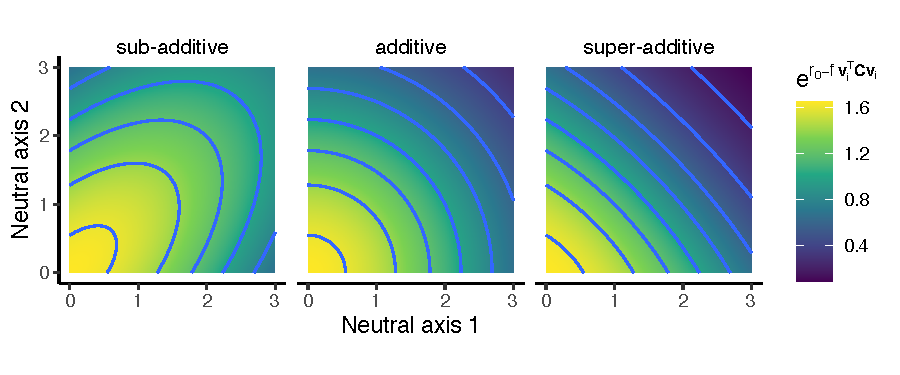
\includegraphics{S1-tradeoffs_r.pdf}
\caption{Costs across axis space, for sub-additive ($\eta = -0.6$), 
additive ($\eta = 0$), and super-additive ($\eta = 0.6$) tradeoffs.
Color indicates the per-capita growth rate without any competition
($\text{e}^{r_0 - f \, \mathbf{v}_i^{\text{T}} \, \mathbf{C} \, \mathbf{v}_i}$),
so darker colors indicate a greater cost.}
\label{fig:tradeoffs-r}
\end{figure}





\begin{figure}[ht!]
\centering
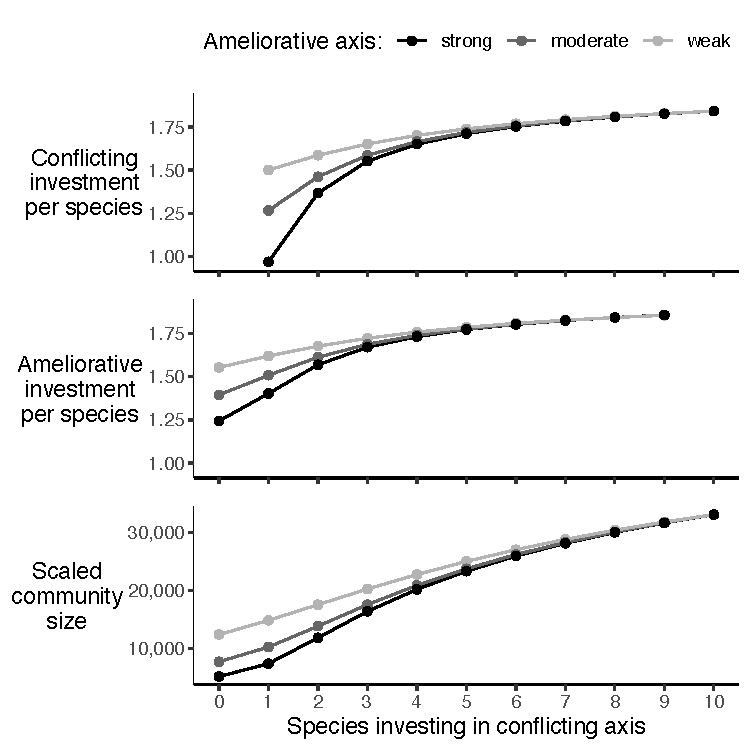
\includegraphics{S2-stab_p2.pdf}
\caption{Effects of the number of species investing in the conflicting axis
in 10-species communities with super-additive tradeoffs on 
(a) conflicting-axis investment per species,
(b) ameliorative-axis investment per species, and 
(c) scaled community size (inversely related to how conducive a community 
is to adding more species).
Color indicates whether the ameliorative axis is strong ($d_{\text{amel}} = 1$),
moderate ($d_{\text{amel}} = 0.5$), or weak ($d_{\text{amel}} = 0.1$).
The conflicting axis was fixed at $d_{\text{conf}} = 0.5$.
}
\label{fig:stabilizers2}
\end{figure}


\begin{figure}[ht!]
\centering
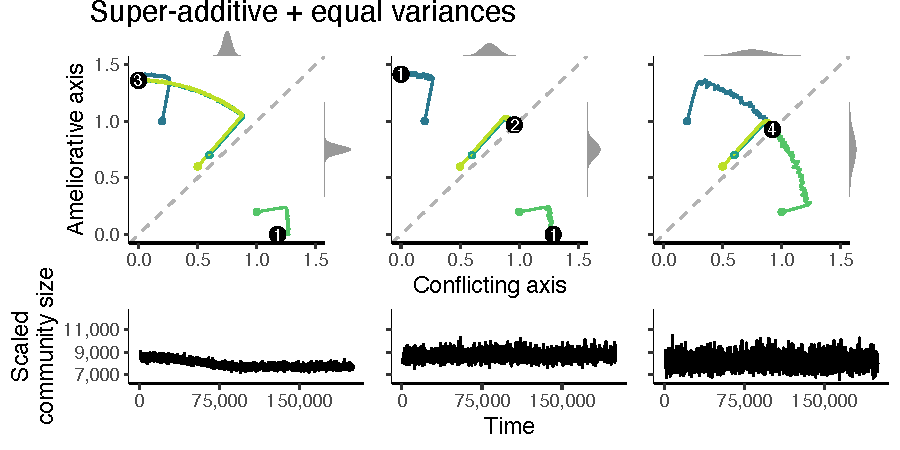
\includegraphics{S3-alt_stoch.pdf}
\caption{Alternative example of how stochasticity affects tradeoffs, 
possible communities, and how conducive communities are to coexistence.
Shown are the effects of axis-evolution stochasticity when
variance is equal among axes and tradeoffs are super-additive.
The upper row shows the trajectories in axis space
for 4 species started under each scenario of stochasticity variances.
Open points indicate starting axis values.
Closed points indicate ending axis values, and 
numbers inside these points indicate the number of species at each point.
Gray shaded curves outside each plot show the probability density for
the normal distributions used to generate stochasticity in the
conflicting (top curve) or ameliorative (right curve) axis.
The lower row shows scaled community size through time for each community
in the top row;
a lower scaled community size indicates that the community is more 
conducive to further species packing.
The first 1,000 time steps are removed to better highlight differences
between communities after the initial period of population expansions.
}
\label{fig:alt-stochasticity}
\end{figure}

